\documentclass[class=report, float=false, crop=false]{standalone}

\usetheme{Warsaw}
% \usecolortheme{spruce}

%%%%% PACKAGES

\usepackage{graphicx} % figures
\usepackage{multimedia} % videos
\usepackage{url}
\usepackage{amsmath}
\usepackage{amssymb}
\everymath{\displaystyle}
\usepackage{epstopdf} % conversion from .eps to .pdf
\usepackage[utf8]{inputenc}
\usepackage[T1]{fontenc}
\usepackage{upgreek}
\usepackage{nameref}
\usepackage{url}
\usepackage{pgf, tikz}
\usepackage{float}
\usepackage[english]{babel}
\usepackage{caption}
\usepackage{subcaption}
\usepackage{fontawesome5}
\usepackage{xcolor}

\usepackage{biblatex}
\addbibresource{references/biblio.bib}

%%%%% TEMPLATE

\captionsetup{font=scriptsize,labelfont={scriptsize, color=blue}}

\AtBeginSubsection[]
{
 \begin{frame}<beamer>{}
   \tableofcontents[currentsection,currentsubsection]
 \end{frame}
}
\AtBeginSection[]
{
  \begin{frame}<beamer>{}
    \tableofcontents[currentsection]
  \end{frame}
}

\defbeamertemplate*{footline}{mytheme}%
{  \begin{beamercolorbox}[ht=2.5ex]{bordure}
\begin{beamercolorbox}[wd=0.2\paperwidth,ht=2.5ex,dp=1ex,center]{author in head/foot}%
\usebeamerfont{author in head}\insertshortauthor
\end{beamercolorbox}%
\begin{beamercolorbox}[wd=0.57\paperwidth,ht=2.5ex,dp=1ex,center]{title in head/foot}%
\usebeamerfont{title in head/foot}\insertshorttitle
\end{beamercolorbox}%
% \begin{beamercolorbox}[wd=0.4\paperwidth,ht=2.5ex,dp=1ex,center]{title in head/foot}%
% \usebeamerfont{title in head/foot}\insertdate
% \end{beamercolorbox}%
\begin{beamercolorbox}[wd=0.12\paperwidth,ht=2.5ex,dp=1ex,center]{title in head/foot}%
\usebeamerfont{title in head/foot}\insertdate
\end{beamercolorbox}%
\begin{beamercolorbox}[wd=0.11\paperwidth,ht=2.5ex,dp=1ex,center]{date in head/foot}%
\usebeamerfont{date in head/foot}\insertframenumber /\inserttotalframenumber{}\hspace{2ex}
\end{beamercolorbox}%

  \end{beamercolorbox}
}

% \defbeamertemplate*{headline}{mytheme}%
% {  \begin{beamercolorbox}[ht=2.5ex]{bordure}
% \begin{beamercolorbox}[wd=\paperwidth,ht=2.5ex,dp=2ex]{author in head/foot}%
% \usebeamerfont{author in head}\vskip6pt\insertsectionnumber.~\insertsection \hfill \insertsubsection
% \end{beamercolorbox}%
%
%   \end{beamercolorbox}
% }

\makeatletter
\let\insertsupervisor\relax
\newcommand\supervisortitle{supervised by}
\mode<all>
{
  \newcommand\supervisor[1]{\def\insertsupervisor{#1}}
  \titlegraphic{}
}
\defbeamertemplate*{title page}{supdefault}[1][]
{
  \vbox{}
  \vfill
  \begingroup
    \centering
    \begin{beamercolorbox}[sep=8pt,center,#1]{title}
      \usebeamerfont{title}\inserttitle\par%
      \ifx\insertsubtitle\@empty\relax%
      \else%
        \vskip0.25em%
        {\usebeamerfont{subtitle}\usebeamercolor[fg]{subtitle}\insertsubtitle\par}%
      \fi%
    \end{beamercolorbox}%
    \vskip1em\par
    \begin{beamercolorbox}[sep=8pt,center,#1]{author}
      \usebeamerfont{author}\textbf{\insertauthor}
    \end{beamercolorbox}
    \vspace{-10pt}
    \ifx\insertsupervisor\relax\relax\else
    \begin{beamercolorbox}[sep=8pt,center,#1]{author}
      \usebeamerfont{author}{\footnotesize \supervisortitle}~{\small\insertsupervisor}
    \end{beamercolorbox}\fi
    \vspace{-5pt}
    \begin{beamercolorbox}[sep=8pt,center,#1]{date}
      \usebeamerfont{date}\insertdate
    \end{beamercolorbox}\vskip0.5em
    {\usebeamercolor[fg]{titlegraphic}\inserttitlegraphic\par}
  \endgroup
  \vfill
}
\setbeamertemplate{title page}[supdefault][colsep=-4bp,rounded=true,shadow=\beamer@themerounded@shadow]\makeatother

\setbeamerfont{footnote}{size=\tiny}

\makeatletter
\newlength\beamerleftmargin
\setlength\beamerleftmargin{\Gm@lmargin}
\makeatother

%%%%% COMMANDS

\providecommand\blfootnote[1]{%
  \begingroup
  \renewcommand\thefootnote{}\footnote{#1}%
  \addtocounter{footnote}{-1}%
  \endgroup
}

\providecommand\encircle[1]{%
  \tikz[baseline=(X.base)]
    \node (X) [draw, shape=circle, inner sep=0] {\strut #1};}

\providecommand{\appropto}{\mathrel{\vcenter{
  \offinterlineskip\halign{\hfil$##$\cr
    \propto\cr\noalign{\kern2pt}\sim\cr\noalign{\kern-2pt}}}}}

\setbeamertemplate{blocks}[rounded][shadow=true]

\providecommand{\isEquivTo}[1]{\underset{#1}{\sim}}

\providecommand{\appropto}{\mathrel{\vcenter{
  \offinterlineskip\halign{\hfil$##$\cr
    \propto\cr\noalign{\kern2pt}\sim\cr\noalign{\kern-2pt}}}}}

\makeatletter
\providecommand{\subalign}[1]{%
  \vcenter{%
    \Let@ \restore@math@cr \default@tag
    \baselineskip\fontdimen10 \scriptfont\tw@
    \advance\baselineskip\fontdimen12 \scriptfont\tw@
    \lineskip\thr@@\fontdimen8 \scriptfont\thr@@
    \lineskiplimit\lineskip
    \ialign{\hfil$\m@th\displaystyle##$&$\m@th\displaystyle{}##$\crcr
      #1\crcr
    }%
  }
}
\makeatother


\graphicspath{{figures/images/}{figures/figs/}}

\begin{document}

\chapter{Shear strain correlation}
\label{chap:strain}

\section{Plastic deformation}
\label{section:plastic_deformation}

Current theories of plastic deformation of amorphous solids rely on the existence of \textit{shear transformation zones}, which are special sites, a few particles wide, where particles are able to rearrange themselves in response to applied stresses \cite{falk1998dynamics}. Plastic deformation is then the consequence of localized irreversible rearrangements, coupled by elastic strain fields \cite{nicolas2014spatiotemporal} which are solutions of the Eshelby inclusion problem \cite{eshelby1959elastic}.\\

These plastic rearrangements, coupled in an elastic medium, have also been observed in supercooled liquids near the glass transition \cite{chattoraj2013elastic, illing2016strain, hassani2018long}, hence the claim that supercooled liquids are "solids that flow" \cite{dyre2006colloquium}.\\

With $\varepsilon_{xy}(\vec{r}, t, t + \Delta t)$ the accumulated shear strain at position $\vec{r}$ and between times $t$ and $t + \Delta t$ (see section \ref{subsection:shear_strain}), we have in these systems that $C_{\varepsilon_{xy}\varepsilon_{xy}}(\Delta \vec{r}, \Delta t)$, its autocorrelation function (see section \ref{subsection:shear_strain_correlation}), has the same quadrupolar symmetry and algebraic decay far from the origin as the strain field \cite{illing2016strain, hassani2018long}, \textit{i.e.}
\begin{equation}
C_{\varepsilon_{xy}\varepsilon_{xy}}(\Delta \vec{r}, \Delta t) \underset{\frac{||\Delta \vec{r}||}{a} \gg 1}{\propto} \frac{\cos4\theta}{||\Delta \vec{r}||^2}
\label{css_eshelby}
\end{equation}
in 2 dimensions, with $a$ the average interparticle distance.\\

In this chapter, we aim at determining if the transition from the fluid to the phase separated regime is associated with the development of algebraic shear strain correlations.

\section{Shear strain}

\subsection{Shear strain}
\label{subsection:shear_strain}

With $\vec{u}(\vec{r}, t, t + \Delta t) = \begin{pmatrix} u_x(\vec{r}, t, t + \Delta t) \\ u_y(\vec{r}, t, t + \Delta t) \end{pmatrix}$ the displacement of particle at position $\vec{r}$ at time $t$ between times $t$ and $t + \Delta t$, we introduce the linearised strain tensor $\rttensor{\varepsilon}$ \cite{landau1986theory}
\begin{equation}
\begin{aligned}
&\rttensor{\varepsilon}(\vec{r}, t, t + \Delta t)\\
\underset{\frac{||\vec{u}||}{L} \ll 1}{=} &\begin{pmatrix} \frac{\partial}{\partial x} u_x(\vec{r}, t, t + \Delta t) & \frac{1}{2} \left(\frac{\partial}{\partial y} u_x(\vec{r}, t, t + \Delta t) + \frac{\partial}{\partial x} u_y(\vec{r}, t, t + \Delta t)\right) \\ \frac{1}{2} \left(\frac{\partial}{\partial y} u_x(\vec{r}, t, t + \Delta t) + \frac{\partial}{\partial x} u_y(\vec{r}, t, t + \Delta t)\right) &  \frac{\partial}{\partial y} u_y(\vec{r}, t, t + \Delta t) \end{pmatrix}
\end{aligned}
\end{equation}
with $L$ the characteristic length of the system, in which we will consider only the diagonal terms, $\textit{i.e.}$ the linearised shear strain
\begin{equation}
\varepsilon_{xy}(\vec{r}, t, t + \Delta t) = \varepsilon_{yx} = \frac{1}{2} \left(\frac{\partial}{\partial y} u_x(\vec{r}, t, t + \Delta t) + \frac{\partial}{\partial x} u_y(\vec{r}, t, t + \Delta t)\right)
\label{linearised_shear_strain}
\end{equation}
which characterises the deformation of the system perpendicularly to the direction of deformation.

\subsection{Shear strain correlation}
\label{subsection:shear_strain_correlation}

We define the shear strain correlation, which is the auto-correlation function of the linearised shear strain introduced in equation \ref{linearised_shear_strain}
\begin{equation}
\begin{aligned}
C_{\varepsilon_{xy}\varepsilon_{xy}}(\Delta \vec{r}, \Delta t) &= \left<\varepsilon_{xy}(\vec{r}+\Delta\vec{r}, t, t + \Delta t)\varepsilon_{xy}(\vec{r}, t, t + \Delta t)\right>_{\vec{r}, t}\\
&= \frac{\int dt \int d^2\vec{r}~ \varepsilon_{xy}(\vec{r}, t, t+\Delta t)\varepsilon_{xy}(\vec{r} + \Delta \vec{r}, t, t+\Delta t)}{\int dt \int d^2\vec{r}~ |\varepsilon_{xy}(\vec{r}, t, t+\Delta t)|^2}\\
&= \frac{\mathcal{F}^{-1}\{\int dt~ |\mathcal{F}\{\varepsilon_{xy}\}(\vec{k}, t, t + \Delta t)|^2\}(\Delta \vec{r}, \Delta t)}{\int dt \int d^2\vec{r}~ ||\varepsilon_{xy}(\vec{r}, t, t+\Delta t)||^2}
\end{aligned}
\label{Css}
\end{equation}
where we refer to appendix \ref{field_auto_correlation} for calculation details leading to the last line of equation \ref{Css}.\\

As discussed in section \ref{section:plastic_deformation}, we expect $C_{\varepsilon_{xy}\varepsilon_{xy}}(\Delta \vec{r}, \Delta t)$ to have a four-fold symmetry. Inspired by \cite{illing2016strain}, we then introduce the projection of the shear strain correlation on $\cos4\theta$
\begin{equation}
C_4^4(\Delta r, \Delta t) = \frac{1}{\pi} \int_0^{2\pi} d\theta~ \cos(4\theta)~ C_{\varepsilon_{xy}\varepsilon_{xy}}(\Delta\vec{r}\equiv(\Delta r, \theta), \Delta t)
\label{c44_definition}
\end{equation}
which in a 2D elastic medium should decay algebraically far from the origin
\begin{equation}
C_4^4(\Delta r, \Delta t) \underset{\frac{\Delta r}{a} \gg 1}{\propto} \frac{1}{\Delta r^2}
\end{equation}
where $a$ is the average interparticle distance.

\section{Real space method}

\subsection{Method}
\label{subsection:real_space_method}

\myparagraph{Coarse-graining}

We only have access to discrete particle positions to calculate displacements. In order to obtain smooth strain fields, we then have to go through some sort of coarse-graining of these displacements.\\

On the basis of a method detailed in \cite{goldhirsch2002microscopic}, we define the coarse-graining operator $\mathcal{A}(\sigma, r_c)$ which associates to any particle-dependent variable $c_i(t)$ its coarse-grained version $\bar{c}(\vec{r}, t)$ such that
\begin{equation}
\bar{c}(\vec{r}, t) = \mathcal{A}(\sigma, r_c)\{c_i(t)\} = \sum_{i=1}^N c_i(t) \phi(\vec{r}-\vec{r}_i(t), \sigma, r_c)
\end{equation}
where $\phi(\vec{r}, \sigma, r_c)$ is a normalised non-negative coarse-graining function, with a single maximum at $\vec{r} = \vec{0}$, of width $\sigma$ -- the coarse-graining scale -- and cut-off radius $r_c$.\\

As has been done in \cite{illing2016strain}, we choose a Gaussian coarse-graining function $\phi(\vec{r}, \sigma, r_c)$ of width $\sigma$ with a cut-off radius $r_c$
\begin{equation}
\phi(\vec{r}, \sigma, r_c) = \frac{1}{\mathcal{N}(\sigma, r_c)} \begin{cases} \exp\left(-\frac{||\vec{r}||^2}{2\sigma^2}\right) &\text{ if } ||\vec{r}|| < r_c \\ 0 & \text{ otherwise} \end{cases}
\end{equation}
where $\mathcal{N}(\sigma, r_c)$ normalises the function, \textit{i.e.} is such that
\begin{equation}
\int_{\mathbb{R}^2} d^2\vec{r}~ \phi(\vec{r}, \sigma, r_c) = \frac{1}{\mathcal{N}(\sigma, r_c)}\int_0^{r_c} dr~ 2 \pi r \exp\left(-\frac{r^2}{2\sigma^2}\right) = 1 \Leftrightarrow \mathcal{N}(\sigma, r_c) = 2\pi\sigma^2\left(1 - \exp\left(-\frac{r_c^2}{2\sigma^2}\right)\right)
\end{equation}
It is straightforward to verify that this coarse-graining function satisfies the aforementioned conditions.\\

We then define the coarse-grained displacement field \cite{illing2016strain}
\begin{equation}
\bar{\vec{u}}(\vec{r}, t, t+\Delta t) = \frac{1}{\bar{\rho}(\vec{r}, t)} \mathcal{A}(\sigma, r_c)\{\vec{u}(\vec{r}_i(t), t, t+\Delta t)\} = \frac{1}{\bar{\rho}(\vec{r}, t)} \sum_{i=1}^N \vec{u}(\vec{r}_i(t), t, t+\Delta t) \phi(\vec{r}-\vec{r}_i(t), \sigma, r_c)
\label{coarse_grained_u}
\end{equation}
where $\bar{\rho}(\vec{r}, t)$ is the coarse-grained density
\begin{equation}
\bar{\rho}(\vec{r}, t) = \mathcal{A}(\sigma, r_c)\{m_i\} = \sum_{i=1}^N m_i \phi(\vec{r}-\vec{r}_i(t), \sigma, r_c)
\end{equation}
with $m_i$ the mass of particle $i$.\\

It follows, from equations \ref{linearised_shear_strain} and \ref{coarse_grained_u}, the expression of the linearised shear strain from the coarse-grained displacements
\begin{equation}
\begin{aligned}
\varepsilon_{xy}(\vec{r}, t, t + \Delta t) &= \frac{1}{2} \left(\frac{\partial}{\partial x}\bar{u}_y(\vec{r}, t, t + \Delta t) + \frac{\partial}{\partial y}\bar{u}_x(\vec{r}, t, t + \Delta t)\right)\\
&= \frac{1}{2}\begin{aligned}[t]\Bigg[&\frac{\partial}{\partial x}\left(\frac{1}{\bar{\rho}(\vec{r}, t)}\right)\underbrace{\sum_{i=1}^N u_y(\vec{r}_i(t), t, t + \Delta t)\phi(\vec{r} - \vec{r}_i(t), \sigma, r_c)}_{\displaystyle\mathcal{A}(\sigma, r_c)\{u_y(\vec{r}_i(t), t, t + \Delta t)\}}\\
&+ \frac{1}{\bar{\rho}(\vec{r}, t)}\sum_{i=1}^N u_y(\vec{r}_i(t), t, t + \Delta t) \frac{\partial}{\partial x}\left(\phi(\vec{r} - \vec{r}_i(t), \sigma, r_c)\right)\\
&+ \frac{\partial}{\partial y}\left(\frac{1}{\bar{\rho}(\vec{r}, t)}\right)\underbrace{\sum_{i=1}^N u_x(\vec{r}_i(t), t, t + \Delta t)\phi(\vec{r} - \vec{r}_i(t), \sigma, r_c)}_{\displaystyle\mathcal{A}(\sigma, r_c)\{u_x(\vec{r}_i(t), t, t + \Delta t)\}}\\
&+ \frac{1}{\bar{\rho}(\vec{r}, t)}\sum_{i=1}^N u_x(\vec{r}_i(t), t, t + \Delta t) \frac{\partial}{\partial x}\left(\phi(\vec{r} - \vec{r}_i(t), \sigma, r_c)\right)\Bigg]\end{aligned}
\end{aligned}
\end{equation}
where we have, $\forall \vec{r}$ such that $||\vec{r}|| < r_c$,
\begin{equation}
\begin{aligned}
\frac{\partial}{\partial \vec{r}}\phi(\vec{r} - \vec{r}_i(t), \sigma, r_c) &= \frac{1}{\mathcal{N}(\sigma, r_c)}\frac{\partial}{\partial\vec{r}} \exp\left(-\frac{||\vec{r} - \vec{r}_i(t)||^2}{2\sigma^2}\right)\\
&= - \frac{\vec{r} - \vec{r}_i(t)}{\mathcal{N}(\sigma, r_c)\sigma^2} \exp\left(-\frac{||\vec{r} - \vec{r}_i(t)||^2}{2\sigma^2}\right)\\
&= - \frac{\vec{r} - \vec{r}_i(t)}{\sigma^2}\phi(\vec{r} - \vec{r}_i(t), \sigma, r_c)
\end{aligned}
\end{equation}
which result can be extrapolated to any $\vec{r}$, and from which it directly follows for any particle-dependent variable $c_i(t)$ that
\begin{equation}
\begin{aligned}
\frac{\partial}{\partial \vec{r}} \bar{c}(\vec{r}, t) &= \sum_{i=1}^N c_i(t) \frac{\partial}{\partial \vec{r}} \phi(\vec{r} - \vec{r}_i(t), \sigma, r_c)\\
&= -\frac{1}{\sigma^2} \sum_{i=1}^N c_i(t) (\vec{r} - \vec{r}_i(t)) \phi(\vec{r} - \vec{r}_i(t), \sigma, r_c)\\
&= -\frac{1}{\sigma^2} \mathcal{A}(\sigma, r_c)\left\{c_i(t)(\vec{r} - \vec{r}_i(t))\right\}
\end{aligned}
\end{equation}
and thus for the coarse-grained density in particular
\begin{equation}
\begin{aligned}
\frac{\partial}{\partial\vec{r}} &= -\frac{1}{\bar{\rho}^2(\vec{r}, t)} \frac{\partial}{\partial\vec{r}} \bar{\rho}(\vec{r}, t)\\
&= \frac{1}{\bar{\rho}^2(\vec{r}, t)\sigma^2} \mathcal{A}(\sigma, r_c)\left\{m_i(\vec{r} - \vec{r}_i(t))\right\}
\end{aligned}
\end{equation}
which finally leads to the expression of the linearised shear strain as function of the positions, masses and displacements of the particles, and the coarse-grained density
\begin{equation}
\begin{aligned}
\varepsilon_{xy}(\vec{r}, t, t + \Delta t) = \frac{1}{2}
&\begin{aligned}[t]\Bigg[\frac{1}{\bar{\rho}^2(\vec{r}, t)\sigma^2} \Big(&\mathcal{A}(\sigma, r_c)\left\{m_i(y - y_i(t))\right\} \times \mathcal{A}(\sigma, r_c)\left\{u_x(\vec{r}_i(t), t, t + \Delta t)\right\} \\ + &\mathcal{A}(\sigma, r_c)\left\{m_i(x - x_i(t))\right\} \times \mathcal{A}(\sigma, r_c)\left\{u_y(\vec{r}_i(t), t, t + \Delta t)\right\}\Big)\end{aligned}\\
& \begin{aligned}[t]-\frac{1}{\bar{\rho}(\vec{r}, t)\sigma^2} \Big(&\mathcal{A}(\sigma, r_c)\left\{u_x(\vec{r}_i(t), t, t + \Delta t)(y - y_i(t))\right\} \\ + &\mathcal{A}(\sigma, r_c)\left\{u_y(\vec{r}_i(t), t, t + \Delta t)(x - x_i(t))\right\}\Big)\Bigg]\end{aligned}
\end{aligned}
\label{linearised_cg_shear_strain}
\end{equation}

\myparagraph{Computation details}

We divide the system square box in $N_{cases} \times N_{cases}$ linearly spaced square boxes with centres $(\vec{R}_{kl})_{1 \leq k,l \leq N_{cases}}$. We then choose $S_{max}$ times $(t_m)_{1 \leq m \leq S_{max}}$, with $\forall m$, $t_m \geq S_{init}$.\\

In our model, we consider $\forall i \in \llbracket 1; N \rrbracket$, $m_i = 1$.\\

We then have $S_{max}$ grids of linearised shear strain $(\varepsilon_{xy,kl}(t_m, t_m + \Delta t))_{1 \leq k, l \leq N_{cases}}$, defined $\forall k,l \in \llbracket 1; N_{cases} \rrbracket$ by
\begin{equation}
\begin{aligned}
\varepsilon_{xy,kl}(t_m, t_m + \Delta t) = \frac{1}{2}
&\begin{aligned}[t]\Bigg[\frac{1}{\bar{\rho}^2(\vec{R}_{kl} ,t_m)\sigma^2} \Big(&\mathcal{A}(\sigma, r_c)\left\{Y_{kl} - y_i(t_m)\right\} \times \mathcal{A}(\sigma, r_c)\left\{u_x(\vec{r}_i(t_m), t_m, t_m + \Delta t)\right\} \\ + &\mathcal{A}(\sigma, r_c)\left\{X_{kl} - x_i(t)\right\} \times \mathcal{A}(\sigma, r_c)\left\{u_y(\vec{r}_i(t_m), t_m, t_m + \Delta t)\right\}\Big)\end{aligned}\\
& \begin{aligned}[t]-\frac{1}{\bar{\rho}(\vec{R}_{kl}, t_m)\sigma^2} \Big(&\mathcal{A}(\sigma, r_c)\left\{u_x(\vec{r}_i(t), t_m, t_m + \Delta t)(Y_{kl} - y_i(t))\right\} \\ + &\mathcal{A}(\sigma, r_c)\left\{u_y(\vec{r}_i(t), t_m, t_m + \Delta t)(X_{kl} - x_i(t))\right\}\Big)\Bigg]\end{aligned}
\end{aligned}
\label{linearised_cg_shear_strain_grid}
\end{equation}
according to equation \ref{linearised_cg_shear_strain}.\\

Since we have a cut-off radius $r_c$, we can resort to neighbour lists to speed up coarse-graining steps, \textit{i.e.} evaluations of $\mathcal{A}(\sigma, r_c)\{\ldots\}$ expressions. We have thus implemented cell lists \cite{frenkel2001understanding}.\\

We can now take the Fourier transforms of the linearised shear strain grids of equation \ref{linearised_cg_shear_strain_grid}
\begin{equation}
(\tilde{\varepsilon}_{xy,kl}(t_m, t_m + \Delta t))_{1 \leq k, l \leq N_{cases}} = \mathcal{F}\left\{(\varepsilon_{xy,pq}(t_m, t_m + \Delta t))_{1 \leq p, q \leq N_{cases}}\right\}(\vec{K}_{kl}, t_m, t_m + \Delta t)
\end{equation}
with $(\vec{K}_{kl})_{1 \leq k, l \leq N_{cases}}$ the grid of wave vectors, then compute the linearised shear strain correlation grid
\begin{equation}
C_{\varepsilon_{xy}\varepsilon_{xy}}(\vec{R}_{kl}, \Delta t) = \frac{\mathcal{F}^{-1}\left\{\left(\sum_m |\tilde{\varepsilon}_{xy,pq}(t_m, t_m + \Delta t)|^2\right)_{1 \leq p, q \leq N_{cases}}\right\}(\vec{R_{kl})}}{\sum_m\sum_{p, q} \varepsilon_{xy, pq}^2(t_m, t_m + \Delta t)}
\end{equation}
\mbox{}\\

Our computation script is available at \href{https://github.com/yketa/active_particles/blob/master/analysis/css.py}{{\faGithub~ yketa/active\_particles/analysis/css.py}}.

\subsection{Results}
\label{subsection:real_method_results}

\myparagraph{High activity ($\text{Pe} > \text{Pe}_t$)}

We investigate shear strain correlations in a system in phase separated state at high activity.\\

We observe in the shear strain map of figure \ref{css_map_real} that the highest values of shear strain in absolute value are found at the interface between the dense fluid and the active gas. This finding is not surprising since we are dealing here with an interface between phases of very different motilities.\\

We then observe in the shear strain correlation map of figure \ref{css_map_real} that $C_{\varepsilon_{xy}\varepsilon_{xy}}(\Delta \vec{r}, \Delta t)$ effectively has a quadropular symmetry as observed in the litterature \cite{illing2016strain, hassani2018long}. This confirms the relevance of the introduction of the $C_4^4(\Delta r, \Delta t)$ function (see equation \ref{c44_definition}).\\

We have graphically checked that there existed a region of the system where an active gas hole never opened and found that it was the case for a square region of centre $(x=-150, y=150)$ and length $L=300$. We have then looked at strain correlations restricted to this area only. We show in figure \ref{css_map_real_quarter} the resulting strain correlation map. By comparison with figure \ref{css_map_real}, we find that the strain correlation map is sharper if active gas holes are removed.\\

We however stress that this kind of manipulation is not possible for all our systems in the phase separated regime. Indeed, just above the transition from fluid states to phase separated states, multiple smaller and transient active gas holes appear in the system. These holes get bigger as the activity increases until, as in the system we are currently strudying, a single hole appears, which size and position hardly vary during the simulation time. This observation has also already been made for other active systems \cite{wysocki2014cooperative, levis2014clustering}.\\

\begin{figure}[H]
\centering
\includegraphics[width=\textwidth]{figures/figs/Cssb_Dk8000_Vj1000_Rg2000_Nq1000_Io5000_Tl1000_Ml1000_Cn5000_RCUTl2000_SIGMl2000.eps}
\vspace{-1cm}
\caption{Shear strain correlations, calculated with the real space method (see section \ref{subsection:real_space_method}), at packing fraction $\phi = 0.80$, self-propelling velocity $\tilde{v} = 1\cdot10^{-2}$, and rotational diffusion rate $\tilde{\nu}_r = 2\cdot10^{—5}$ (phase separated regime). We have the average particle separation $a \approx 2$. \textbf{(left)} Shear strain map, $\varepsilon_{xy}(\vec{r} \equiv (x, y), t, t + \Delta t)$. There is an open active gas hole in the system, visible on the top and bottom right corners. \textbf{(right)} Shear strain correlation map, $C_{\varepsilon_{xy}\varepsilon_{xy}}(\Delta\vec{r} \equiv (x, y), \Delta t)$.}
\label{css_map_real}
\end{figure}

\begin{figure}[H]
\centering
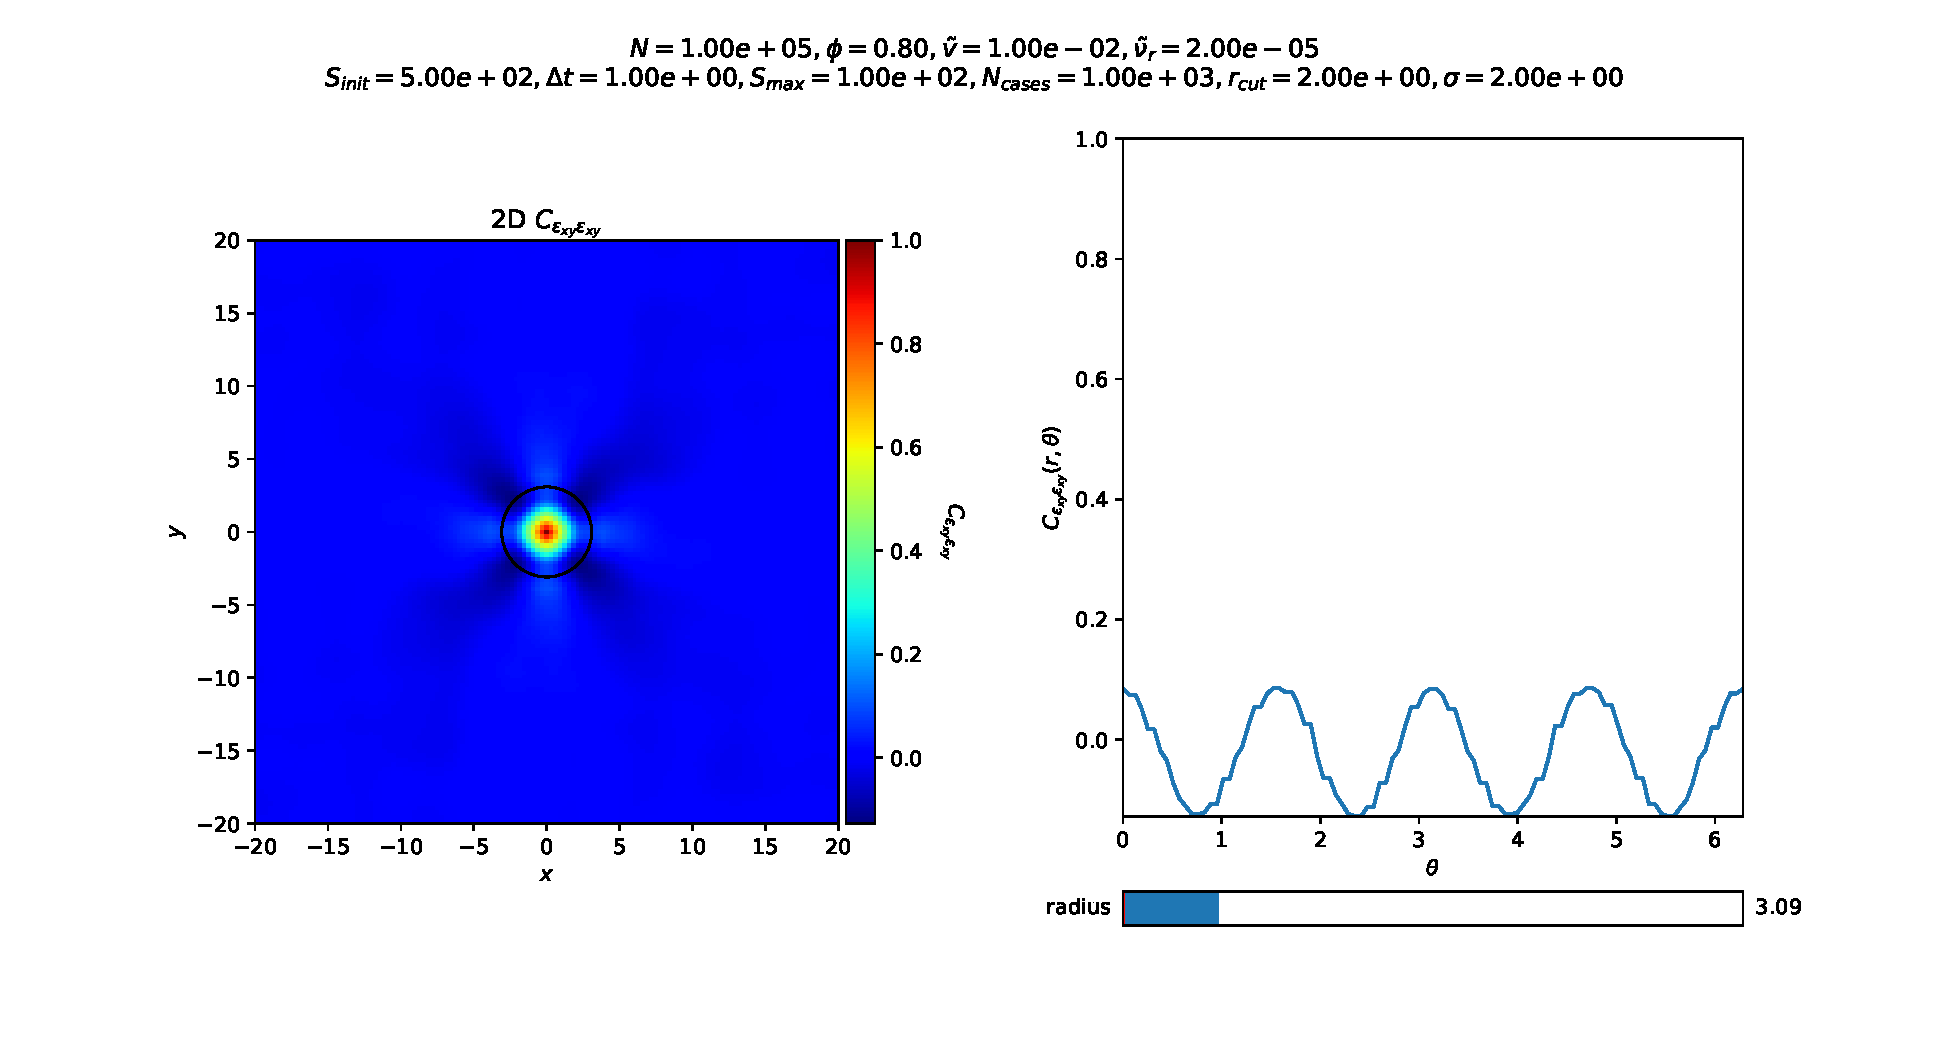
\includegraphics[width=\textwidth]{figures/figs/Cssb_Dk8000_Vj1000_Rg2000_Nq1000_In5000_Tl1000_Ml1000_Co1000_Bn3000_XN1500_Yn1500_grid_circle.eps}
\caption{Shear strain correlations, calculated with the real space method (see section \ref{subsection:real_space_method}), at packing fraction $\phi = 0.80$, self-propelling velocity $\tilde{v} = 1\cdot10^{-2}$, and rotational diffusion rate $\tilde{\nu}_r = 2\cdot10^{—5}$ (phase separated regime), from the square box of centre $(x=-150, y=150)$ and length $L=300$ in the system of figure \ref{css_map_real}. We have the average particle separation $a \approx 2$. \textbf{(left)} Shear strain correlation map, $C_{\varepsilon_{xy}\varepsilon_{xy}}(\Delta\vec{r} \equiv (x, y), \Delta t)$. The black circle materialises the radial projection of the shear strain correlation. \textbf{(right)} Radial projection of the shear strain correlation on a circle of radius $r=3.09$, $C_{\varepsilon_{xy}\varepsilon_{xy}}(\Delta\vec{r} \equiv (r=3.09, \theta), \Delta t)$.}
\label{css_map_real_quarter}
\end{figure}

We calculated shear strain correlations $C_{\varepsilon_{xy}\varepsilon_{xy}}(\Delta \vec{r}, \Delta t)$ for the subsystem of figure \ref{css_map_real_quarter} at different lag times $\Delta t$, then projected them on $\cos4\theta$ according to equation \ref{c44_definition} to obtain $C_4^4(\Delta r, \Delta t)$. These are shown in figure \ref{c44_real}.\\

Our curves are quite similar to the equivalent ones reported in \cite{illing2016strain, hassani2018long}. We have a peak of $C_4^4(\Delta r, \Delta t)$ close to 2 units of average particle separation and curves collapse, at least for $nD_0\Delta t \lessapprox 30$. Our most revelant observation is that our curves are quite consistent with an algebraic decay $(r/a)^{—2}$, indicating scale free correlations reminiscent of a glass-forming material at low temperature, as discussed in section \ref{section:plastic_deformation}.\\

We however have smooth but large fluctuations around this fit, which origin is still unknowsn.\\

\begin{figure}[H]
\centering
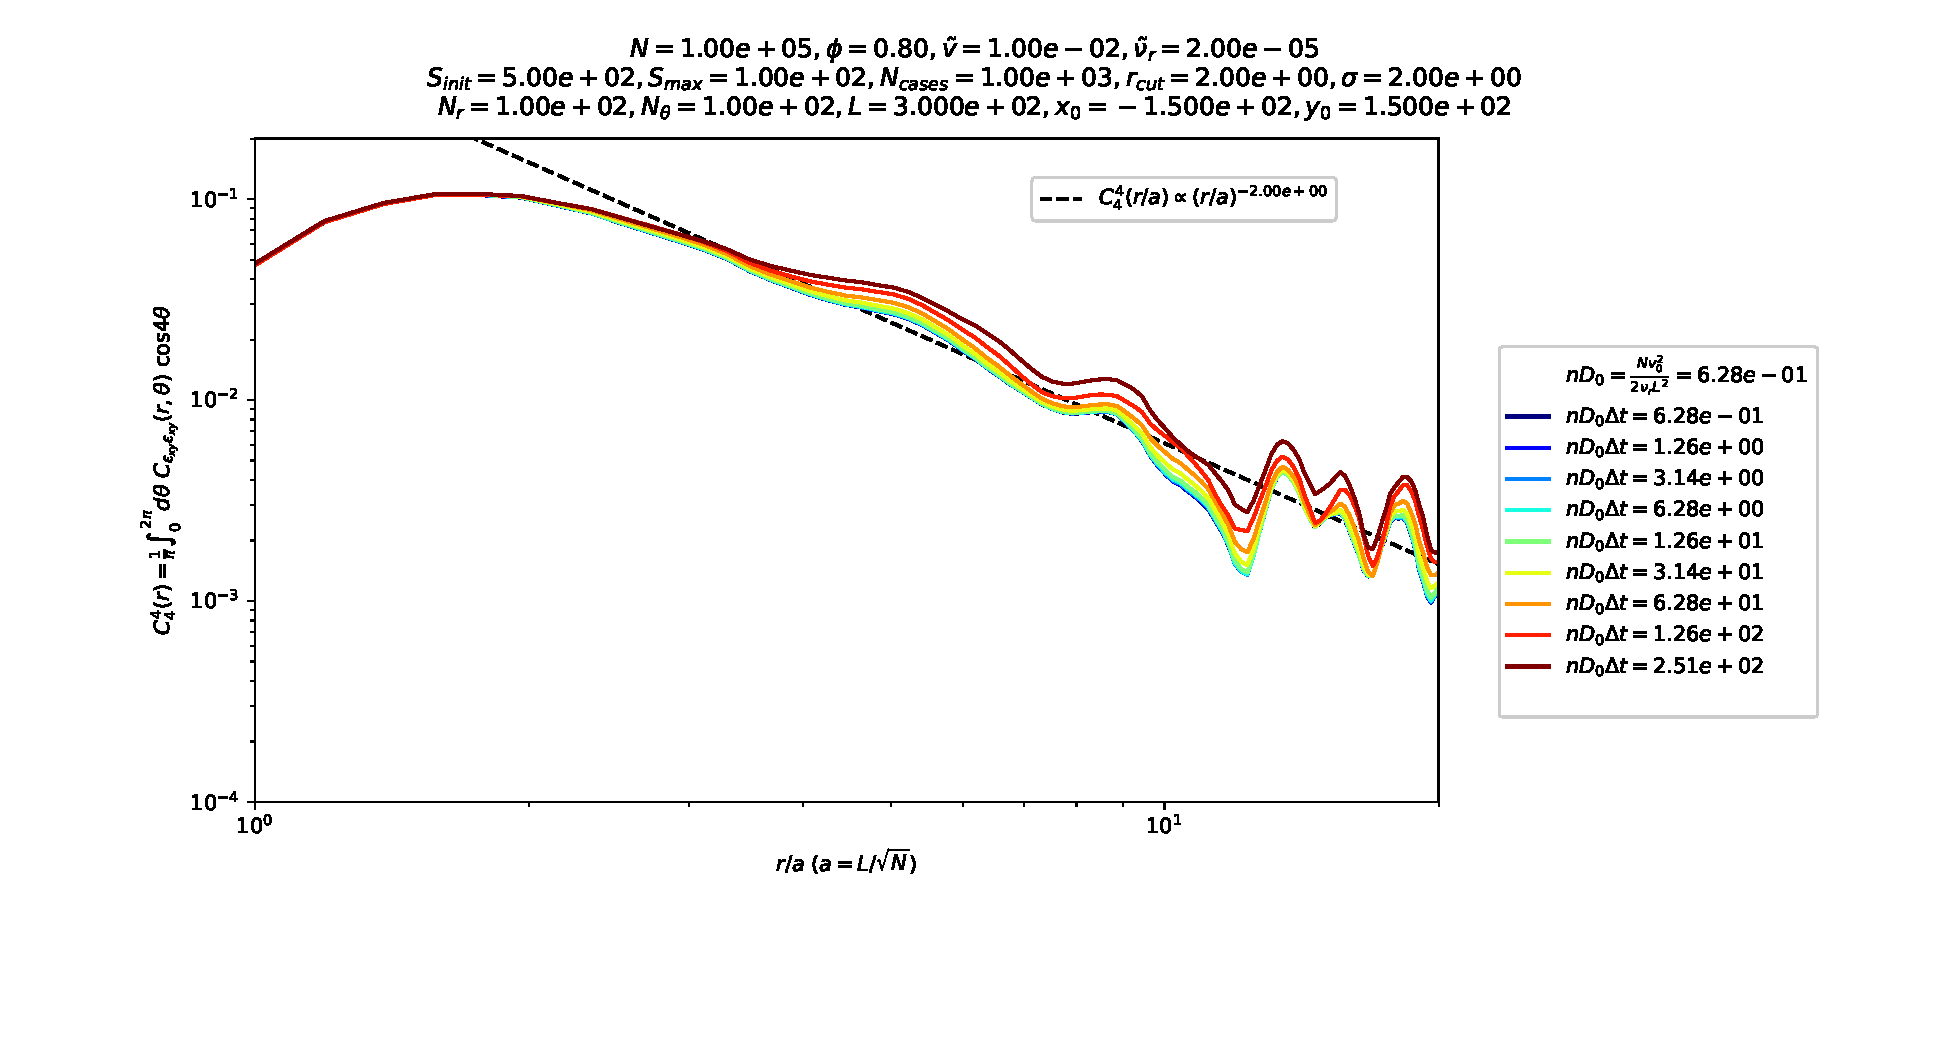
\includegraphics[width=\textwidth]{c44_comparison_Dk8000_Vj1000_Rg2000_Nq1000_Ll2000.eps}
\caption{Projection of shear strain correlations on $\cos4\theta$, $C_4^4(\Delta r, \Delta t)$, according to equation \ref{c44_definition}, at packing fraction $\phi = 0.80$, self-propelling velocity $\tilde{v} = 1\cdot10^{-2}$, and rotational diffusion rate $\tilde{\nu}_r = 2\cdot10^{—5}$ (phase separated regime), for a subsystem containing no active gas holes, for different lag times $\Delta t$. We have $n = N/L^2$ the number density of particles and $D_0 = V_0^2/2\nu_r$ the diffusion constant of a single particle, introduced for matter of comparison of lag times between different systems as suggested in \cite{illing2016strain}. The dashed line corresponds to an arbitrary fit to a power law $(r/a)^{—2}$.}
\label{c44_real}
\end{figure}

\myparagraph{Low activity ($\text{Pe} < \text{Pe}_t$)}

We calculated shear strain correlations $C_{\varepsilon_{xy}\varepsilon_{xy}}(\Delta \vec{r}, \Delta t)$ for a system in fluid state, at different lag times $\Delta t$, then projected them on $\cos4\theta$ according to equation \ref{c44_definition} to obtain $C_4^4(\Delta r, \Delta t)$. These are shown in figure \ref{c44_real_fluid}.\\

We still observe a peak of $C_4^4(\Delta r, \Delta t)$ close to 2 units of average particle separation, however, contrarily to the phase separated state (see figure \ref{c44_real}), we observe here an exponential decay of the shear strain correlation, which length scale is approximately equal to 2 units of average particle separation. A simple exponential decay of correlations is indeed what we would expect in a liquid above the melting point \cite{debenedetti2001supercooled}. We finally add that the length scale of this decay increases sensitively with increasing lag time $\Delta t$.\\

There must then be a transition from an exponential to an algebraic decay of shear strain correlations as activity increases which we need to characterise.

\begin{figure}[H]
\centering
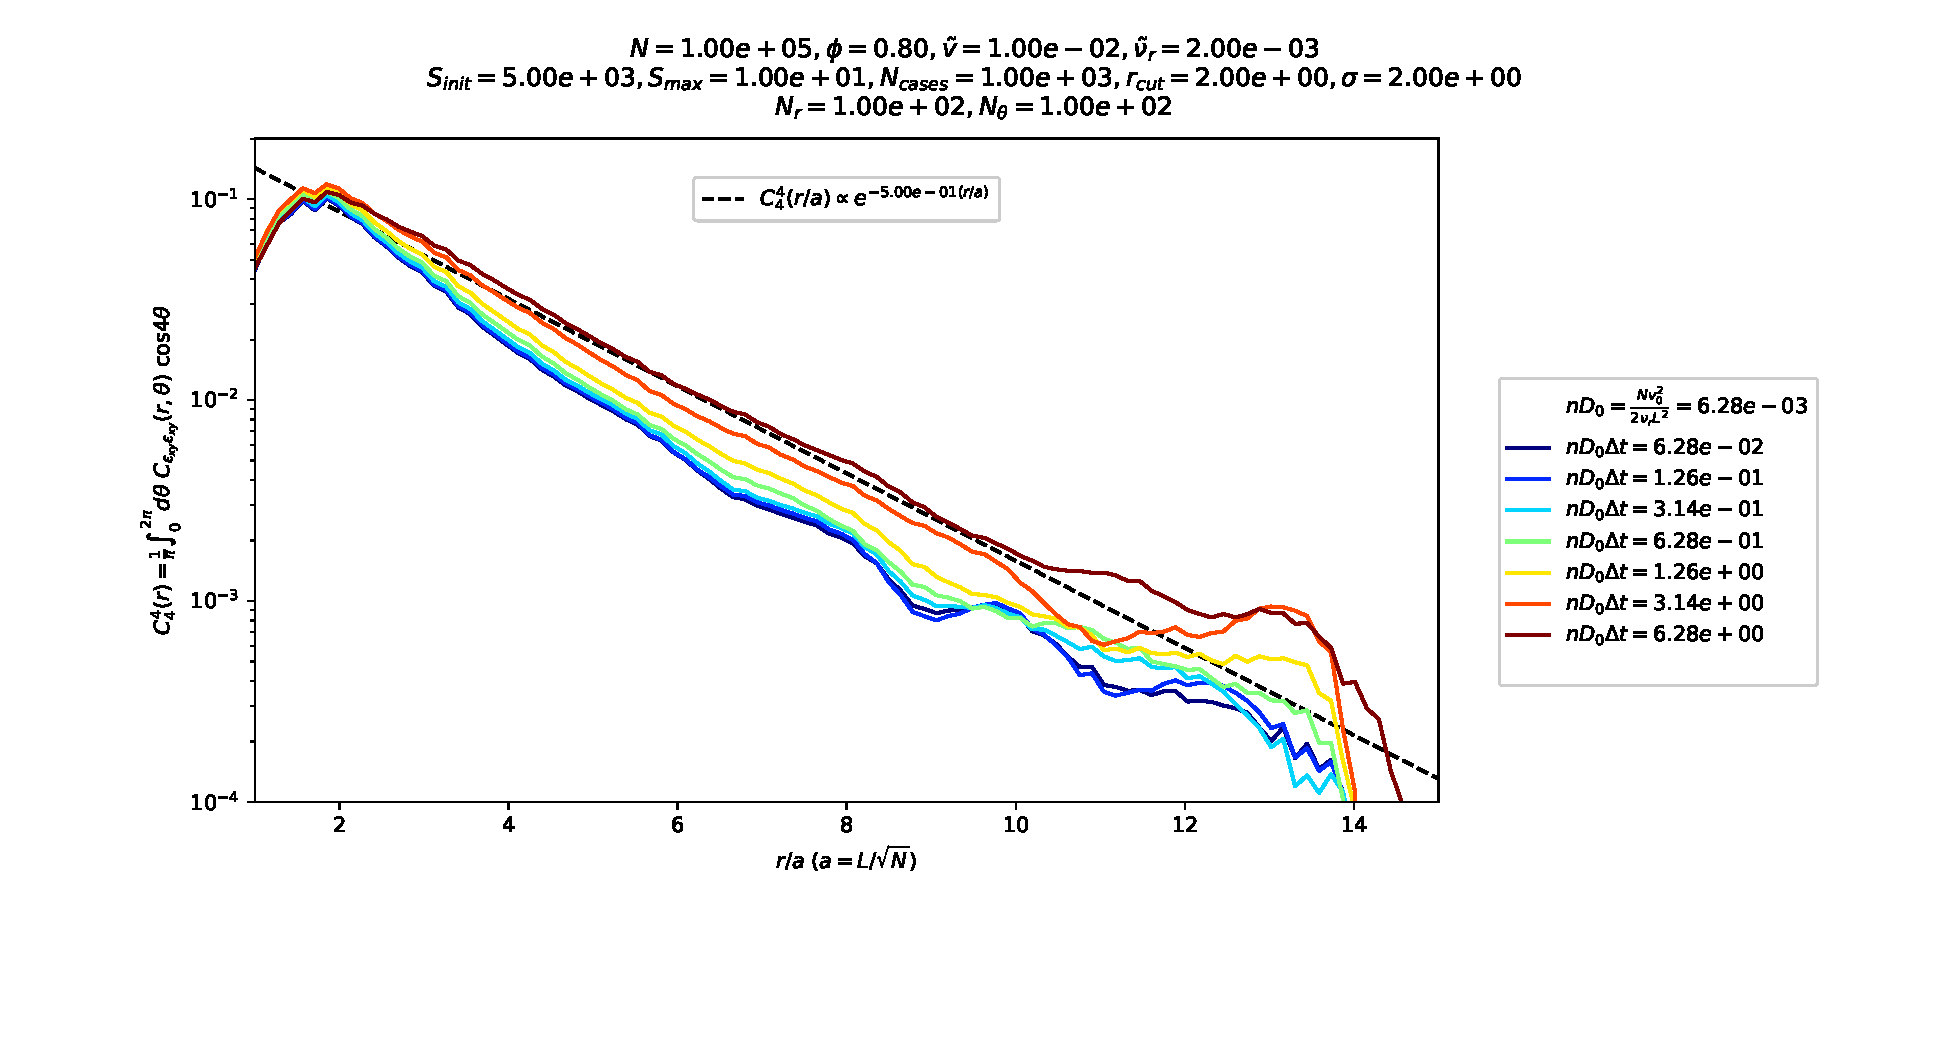
\includegraphics[width=\textwidth]{c44_comparison_Dk8000_Vj1000_Ri2000_Nq1000_Ll0000.eps}
\caption{Projection of shear strain correlations on $\cos4\theta$, $C_4^4(\Delta r, \Delta t)$, according to equation \ref{c44_definition}, at packing fraction $\phi = 0.80$, self-propelling velocity $\tilde{v} = 1\cdot10^{-2}$, and rotational diffusion rate $\tilde{\nu}_r = 2\cdot10^{—3}$ (fluid regime), for different lag times $\Delta t$. We have $n = N/L^2$ the number density of particles and $D_0 = V_0^2/2\nu_r$ the diffusion constant of a single particle, introduced for matter of comparison of lag times between different systems as suggested in \cite{illing2016strain}. The dashed line corresponds to an arbitrary fit to an exponential $\exp(-r/2a)$.}
\label{c44_real_fluid}
\end{figure}

\myparagraph{Issue}

Despite this method giving interesting and encouraging results, we deplore its exceptional slowliness despite our best computational efforts. We introduce in section \ref{section:collective_mean_square_displacement_method} new quantities enabling us to compute shear strain correlations more quickly and efficiently.

\section{Collective mean square displacement method}
\label{section:collective_mean_square_displacement_method}

\subsection{Collective mean square displacement}

\myparagraph{Definition}

We take the Fourier transform of the displacement of the particle at position $\vec{r}$ at time $t$ between times $t$ and $t + \Delta t$, evaluated at wave vector $\vec{k}$ such that $k = ||\vec{k}|| \neq 0$
\begin{equation}
\tilde{\vec{u}}(\vec{k}, t, t + \Delta t) = \mathcal{F}\{\vec{u}(\vec{r}, t, t + \Delta t)\}(\vec{k})
\end{equation}
and introduce
\begin{equation}
\begin{aligned}
\vec{e}_{||} &= \vec{k}/k &&~\parallelsum \vec{k}\\
\vec{e}_{\perp} &= (\vec{e}_z\wedge\vec{k})/k &&\perp \vec{k}
\end{aligned}
\end{equation}
with $\phi = (\vec{e}_x ; \vec{e}_{||})$, such that we can decompose $\tilde{\vec{u}}(\vec{k}, t, t + \Delta t)$ in this base \cite{stackexchange}
\begin{equation}
\begin{aligned}
\begin{pmatrix} \tilde{u}_x(\vec{k}, t, t + \Delta t) \\ \tilde{u}_y(\vec{k}, t, t + \Delta t) \end{pmatrix} &= \begin{pmatrix} \cos\phi & -\sin\phi \\ \sin\phi & \cos\phi \end{pmatrix} \begin{pmatrix} \tilde{u}_{||}(\vec{k}, t, t + \Delta t) \\ \tilde{u}_{\perp}(\vec{k}, t, t + \Delta t) \end{pmatrix}\\
&= \begin{pmatrix} k_x/k & -k_y/k \\ k_y/k & k_x/k \end{pmatrix} \begin{pmatrix} \tilde{u}_{||}(\vec{k}, t, t + \Delta t) \\ \tilde{u}_{\perp}(\vec{k}, t, t + \Delta t) \end{pmatrix}
\label{u_cmsd}
\end{aligned}
\end{equation}
\mbox{}\\

With these notations, we introduce the longitudinal and transversal mean square displacements \cite{illing2016strain, klix2012glass}, respectively $C^{||}(k, \Delta t)$ and $C^{\perp}(k, \Delta t)$, defined by
\begin{equation}
\begin{aligned}
C^{||}(k, \Delta t) &= \left<|\tilde{u}_{||}(\vec{k}, t, t + \Delta t)|^2\right>\\
C^{\perp}(k, \Delta t) &= \left<|\tilde{u}_{\perp}(\vec{k}, t, t + \Delta t)|^2\right>
\end{aligned}
\label{cmsd_definition}
\end{equation}
where $\left<\ldots\right>$ denotes an average over time $t$ and directions of $\vec{k}$ at fixed norm $k$. These functions are collective and spatially resolved generalisations of the mean square displacement \cite{illing2016strain}.\\

We note in \cite{illing2016strain} that for an incompressible glass
\begin{equation}
\begin{aligned}
C^{||}(k, \Delta t) &= 0\\
C^{\perp}(k, \Delta t) \underset{\frac{2\pi}{k} \gg a}&{\propto} k^{-2}
\end{aligned}
\end{equation}
with $a$ the average interparticle distance. Authors of \cite{leonforte2005continuum} also report
\begin{equation}
\begin{aligned}
C^{||}(k, \Delta t) \underset{\frac{2\pi}{k} \gg a}&{\propto} k^{-2}\\
C^{\perp}(k, \Delta t) \underset{\frac{2\pi}{k} \gg a}&{\propto} k^{-2}
\end{aligned}
\end{equation}
in a polydisperse Lennard-Jones mixture under shear.

\myparagraph{Shear strain correlation}

We have from \cite{illing2016strain} a simple relation between shear strain correlations and collective mean square displacements
\begin{equation}
C_{\varepsilon_{xy}\varepsilon_{xy}}(\Delta \vec{r}, \Delta t) = \mathcal{F}^{-1}\left\{-\frac{k_x^2k_y^2}{k^2}\left(C^{\perp}(k, \Delta t) - C^{||}(k, \Delta t)\right) + \frac{k^2}{4}C^{\perp}(k, \Delta t)\right\}(\Delta \vec{r})
\label{css_cmsd}
\end{equation}
hence our interest in these functions.\\

This relation can be derived from
\begin{equation}
C_{\varepsilon_{xy}\varepsilon_{xy}}(\Delta \vec{r}, \Delta t) = \mathcal{F}^{-1}\left\{\left<|\mathcal{F}\left\{\varepsilon_{xy}(\vec{r}, t, t + \Delta t)\right\}(\vec{k})|^2\right>_t\right\}(\Delta \vec{r})
\label{css_from_ft}
\end{equation}
according to appendix \ref{field_auto_correlation}, in which we can replace $u_x(\vec{r}, t, t + \Delta t)$ and $u_y(\vec{r}, t, t + \Delta t)$ by their expressions in terms of $\tilde{u}_{||}(\vec{k}, t, t + \Delta t)$ and $\tilde{u}_{\perp}(\vec{k}, t, t + \Delta t)$ with equation \ref{u_cmsd}, leading to equation \ref{css_cmsd} \cite{stackexchange}.

\myparagraph{Computation details}

First of all, we can note that
\begin{equation}
\begin{aligned}
C^{||}(k, \Delta t) &= \frac{1}{k^2}\left<|\vec{k}\cdot\tilde{\vec{u}}(\vec{k}, t, t + \Delta t)|^2\right>\\
C^{\perp}(k, \Delta t) &= \frac{1}{k^2}\left<||\vec{k}\wedge\tilde{\vec{u}}(\vec{k}, t, t + \Delta t)||^2\right>
\end{aligned}
\label{cmsd_k}
\end{equation}
which expression are used in \cite{leonforte2005continuum}.\\

We divide the system square box in $N_{cases} \times N_{cases}$ linearly spaced square boxes with centres $(\vec{R}_{kl})_{1 \leq k, l \leq N_{cases}}$. With $dL$ the length of each box, we introduce
\begin{equation}
\vec{u}_{kl}(t, t + \Delta t) = \text{mean}\left(\left\{\vec{u}(\vec{r}_i(t), t, t + \Delta t), ||\vec{r}_i(t) - \vec{R}_{kl}||_{+\infty} \leq \frac{dL}{2}\right\}\right)
\end{equation}
the average displacement of particles in each box between times $t$ and $t + \Delta t$. We then choose $S_{max}$ times $(t_m)_{1 \leq m \leq S_{max}}$, with $\forall m, t_m \geq S_{init}$.\\

We now have $\forall m$, a displacement grid $(\vec{u}_{kl}(t_m, t_m + \Delta t))_{1 \leq k, l \leq N_{cases}}$ of which we can take the Fast Fourier Transform
\begin{equation}
(\tilde{\vec{u}}_{kl}(t_m, t_m + \Delta t))_{1 \leq k, l \leq N_{cases}} = \mathcal{F}\left\{(\vec{u}_{pq}(t_m, t_m + \Delta t))_{1 \leq p, q \leq N_{cases}}\right\}(\vec{K}_{kl}, t_m, t_m + \Delta t)
\end{equation}
with $(\vec{K}_{kl})_{1 \leq k, l \leq N_{cases}}$ the grid of wave vectors, then compute the collective mean square displacements
\begin{equation}
\begin{aligned}
C^{\perp}(\vec{K}_{kl}, \Delta t) &= \frac{1}{S_{max}||\vec{K}_{kl}||^2}\sum_m ||\vec{K}_{kl}\wedge\tilde{\vec{u}}_{kl}(t_m, t_m + \Delta t) ||^2\\
C^{||}(\vec{K}_{kl}, \Delta t) &= \frac{1}{S_{max}||\vec{K}_{kl}||^2}\sum_m |\vec{K}_{kl}\cdot\tilde{\vec{u}}_{kl}(t_m, t_m + \Delta t)|^2
\end{aligned}
\end{equation}
according to equation \ref{cmsd_k}. Please note that these functions are slightly different than the one introduced in equation \ref{cmsd_definition} since they now depend on the wave vector rather than its sole norm. We have verified than either definitions gave consistent results and kept this version for algorithmic simplicity.\\

We can then compute the Fourier transform of the shear strain correlation
\begin{equation}
F_{kl}(\Delta t) = -\frac{K_{kl,x}^2K_{kl,y}^2}{K_{kl}^2}\left(C^{\perp}(\vec{K}_{kl}, \Delta t) - C^{||}(\vec{K}_{kl}, \Delta t)\right) + \frac{K_{kl}^2}{4}C^{\perp}(\vec{K}_{kl}, \Delta t)
\label{css_ft}
\end{equation}
according to equation \ref{css_cmsd}, and finally obtain the shear strain correlation through inverse Fast Fourier Transform
\begin{equation}
C_{\varepsilon_{xy}\varepsilon_{xy}}(\vec{R}_{kl}, \Delta t) = \frac{\mathcal{F}^{-1}\left\{\left(F_{pq}(\Delta t)\right)_{1 \leq p, q \leq N_{cases}}\right\}(\vec{R}_{kl})}{\mathcal{F}^{-1}\left\{\left(F_{pq}(\Delta t)\right)_{1 \leq p, q \leq N_{cases}}\right\}(\vec{0})}
\end{equation}
\mbox{}

Our computation script is available at \href{https://github.com/yketa/active_particles/blob/master/analysis/ctt.py}{{\faGithub~ yketa/active\_particles/analysis/ctt.py}}.

\subsection{Results}

\myparagraph{Preliminary results}

First of all, we point out that computing collective mean square displacements is orders of magnitude quicker than computing coarse-grained displacements as described in section \ref{subsection:real_space_method}. This method then seems better suited to systematically analyse shear strain correlations within our model.

\begin{figure}[H]
\centering
\includegraphics[width=\textwidth]{Cttb_Dk8000_Vj1000_Rg2000_Nq1000_Io5000_Tl1000_Mn1000_Cn5000_Bn3000_XN1500_Yn1500.eps}
\vspace{-1cm}
\caption{Collective mean square displacements according to equation \ref{cmsd_definition}, at packing fraction $\phi = 0.80$, self-propelling velocity $\tilde{v} = 1\cdot10^{-2}$, and rotational diffusion rate $\tilde{\nu}_r = 2\cdot10^{—5}$ (phase separated regime). Dashed lines correspond to arbitrary fits to a power law $\lambda^2$. \textbf{(top left)} Transversal collective mean square displacemnt $C^{\perp}(k, \Delta t) = \left<||\vec{k}\wedge\tilde{\vec{u}}(\vec{k}, t, t + \Delta t)||^2\right>$ as function of the wavelength $\lambda = 2\pi/k$. \textbf{(bottom left)} Longitudinal collective mean square displacemnt $C^{||}(k, \Delta t) = \left<|\vec{k}\cdot\tilde{\vec{u}}(\vec{k}, t, t + \Delta t)|^2\right>$ as function of the wavelength $\lambda = 2\pi/k$. \textbf{(right)} Superimposition of the transversal \textit{(blue)} and longitudinal \textit{(orange)} collective mean square displacements.}
\label{preliminary_cmsd}
\end{figure}

We first calculated collective mean square displacements in a system in the phase separated state. This calculation has been performed on the whole system, \textit{i.e.} including the active gas phase. We present our results in figure \ref{preliminary_cmsd}.\\

We observe in figure \ref{preliminary_cmsd} that the longitudinal collective mean square displacement $C^{||}(k, \Delta t)$ is a strictly positive function, indicating that our system is compressible \cite{illing2016strain} which was an expected finding. We however note that the longitudinal part $C^{||}(k, \Delta t)$ is about an order of magnitude lesser than the transversal part $C^{\perp}(k, \Delta t)$ of the collective mean square displacement, as reported in \cite{leonforte2005continuum}.\\

Both $C^{||}(k, \Delta t)$ and $C^{\perp}(k, \Delta t)$ are quite well fitted with a power law $k^{-2}$ for about a decade ($10 \lessapprox \lambda = 2\pi/k \lessapprox 20$), which was also reported in \cite{leonforte2005continuum} and may indicate elastic properties of the system. This algebraic behaviour is limited at high wavelengths by finite-size effects and at low wavelengths by the discrete microscopic structure of the system. Indeed, we have that the peak in both $C^{||}(k, \Delta t)$ and $C^{\perp}(k, \Delta t)$ at $\lambda = 2\pi/k \approx a \approx 2$ with $a$ the average particle separation is a consequence of the discreteness of the displacement field.

\begin{figure}[H]
\centering
\includegraphics[width=\textwidth]{Cttb_Dk8000_Vj1000_Ri7000_Nq1000_Io5000_Tl1000_Mn1000_Cn5000.eps}
\caption{Collective mean square displacements according to equation \ref{cmsd_definition}, at packing fraction $\phi = 0.80$, self-propelling velocity $\tilde{v} = 1\cdot10^{-2}$, and rotational diffusion rate $\tilde{\nu}_r = 7\cdot10^{—3}$ (fluid regime). Dashed lines correspond to arbitrary fits to a power law $\lambda$. \textbf{(top left)} Transversal collective mean square displacemnt $C^{\perp}(k, \Delta t) = \left<||\vec{k}\wedge\tilde{\vec{u}}(\vec{k}, t, t + \Delta t)||^2\right>$ as function of the wavelength $\lambda = 2\pi/k$. \textbf{(bottom left)} Longitudinal collective mean square displacemnt $C^{||}(k, \Delta t) = \left<|\vec{k}\cdot\tilde{\vec{u}}(\vec{k}, t, t + \Delta t)|^2\right>$ as function of the wavelength $\lambda = 2\pi/k$. \textbf{(right)} Superimposition of the transversal \textit{(blue)} and longitudinal \textit{(orange)} collective mean square displacements.}
\label{preliminary_cmsd_low_activity}
\end{figure}

We then calculated collective mean square displacements in a system in the fluid state. We present our results in figure \ref{preliminary_cmsd_low_activity}.\\

As in the high activity case (see figure \ref{preliminary_cmsd}), we observe that the longitudinal collective mean square displacement $C^{||}(k, \Delta t)$ is a strictly positive function. Nonetheless, we notice in this low activity case that the values of $C^{||}(k, \Delta t)$ and $C^{\perp}(k, \Delta t)$ are of the same order of magnitude.\\

Both $C^{||}(k, \Delta t)$ and $C^{\perp}(k, \Delta t)$ are quite well fitted with a power law $k^{-1}$ for about a decade ($6 \lessapprox \lambda = 2\pi/k \lessapprox 60$). However, this exponent for the power law decay of the collective mean square displacements with increasing wave vector norm is puzzling and further investigations are needed to understand it.

\newpage
\myparagraph{Necessity of filtering}

We use the collective mean square displacements presented in figure \ref{preliminary_cmsd} to compute shear strain correlations $C_{\varepsilon_{xy}\varepsilon_{xy}}(\Delta \vec{r}, \Delta t)$ according to equation \ref{css_cmsd}. Our results are presented in figure \ref{non_filtered_css}.

\begin{figure}[H]
\centering
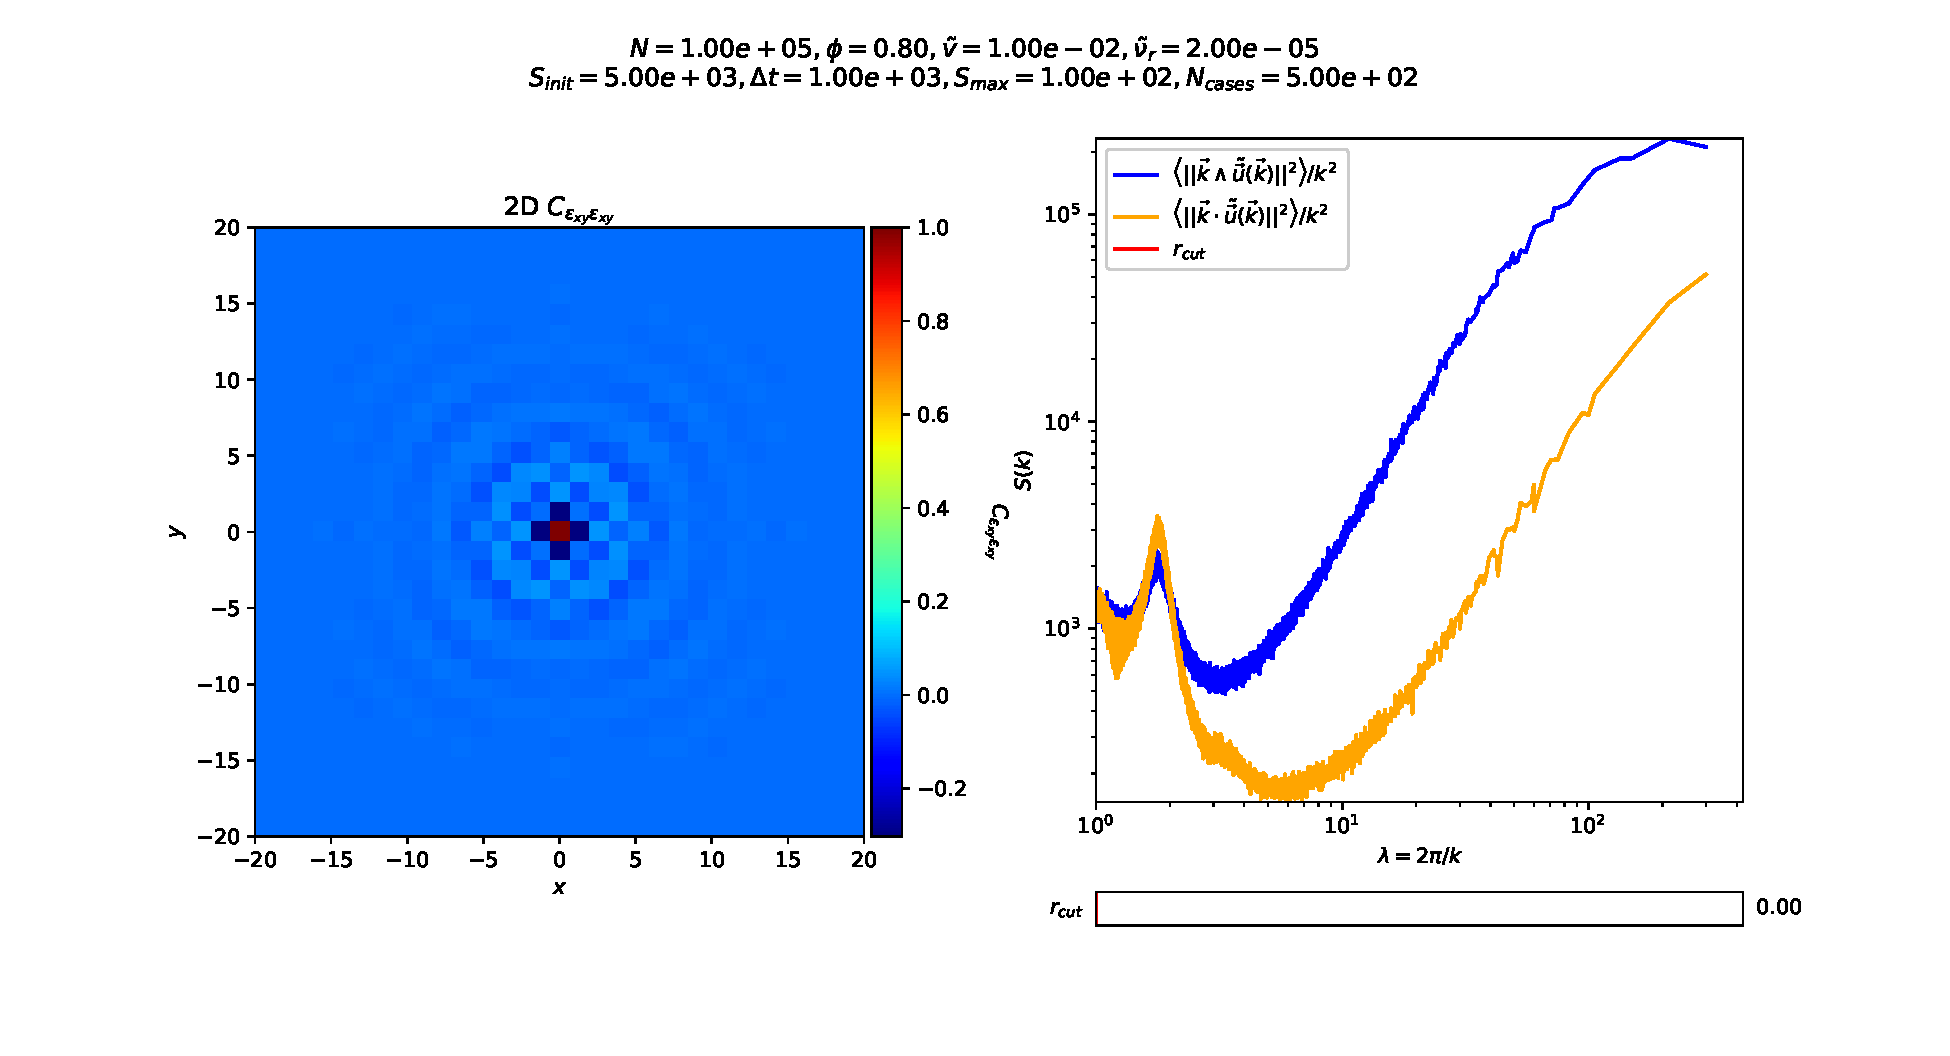
\includegraphics[width=\textwidth]{Cttb_Dk8000_Vj1000_Rg2000_Nq1000_Io5000_Tl1000_Mn1000_Cn5000_Bn3000_XN1500_Yn1500_strain_correlations_RCUTl0000.eps}
\caption{}
\label{non_filtered_css}
\end{figure}

We have that shear strain correlations are completely drowned under a pattern of concentric waves which spatial period is close to the average particle separation $a \approx 2$. As we had discussed on figure \ref{cuu_oscillations}, these waves originate from the fact that our griding is so tight that we are resolving the microscopic structure of the system. This is visible in the collective mean displacement curves (figures \ref{preliminary_cmsd} and \ref{preliminary_cmsd_low_activity}) in the form of a peak near $\lambda = a$.\\

As a solution to this inconvenience, we propose to filter out low wavelengths corresponding to the microscopic structure. This is a form of coarse-graining since it means to eliminate short range degrees of freedom. A first attempt has been to set all Fourier components under a given wavelength to 0, yet this was doomed to failure since completely depriving a signal of its high frequency components is a cause of ringing artifacts \cite{ringing}. A better solution is to perform, as we have done for displacements in the real space methode (see section \ref{subsection:real_space_method}), a Gaussian coarse-graining of the shear strain.\\

We introduce the Gaussian filtering function
\begin{equation}
\mathcal{G}(\vec{r}, r_c) = \frac{1}{2\pi\sigma^2}\exp\left(-\frac{||\vec{r}||^2}{2\sigma^2}\right)
\end{equation}
where $r_c$ is the spatial extent of the function, such that the coarse-grained version of the shear strain, $\varepsilon_{xy}^{(cg)}(\vec{r}, t, t + \Delta t)$, is obtained by convolution
\begin{equation}
\varepsilon_{xy}^{(cg)}(\vec{r}, t, t + \Delta t) = \int_{\mathbb{R}^2} d^2\vec{r}^{\prime}~ \mathcal{G}(\vec{r}^{\prime} - \vec{r}, r_c) \varepsilon_{xy}^{(cg)}(\vec{r}^{\prime}, t, t + \Delta t) = \left[\mathcal{G}\ast\varepsilon_{xy}\right](\vec{r}, t, t + \Delta t)
\end{equation}
\mbox{}\\

We thus obtain in equation \ref{css_from_ft}, when deriving shear strain correlations from coarse-grained shear strain
\begin{equation}
\begin{aligned}
C_{\varepsilon_{xy}\varepsilon_{xy}}(\Delta \vec{r}, \Delta t) &= \mathcal{F}^{-1}\left\{\left<|\mathcal{F}\left\{\varepsilon_{xy}^{(cg)}(\vec{r}, t, t + \Delta t)\right\}(\vec{k})|^2\right>_t\right\}(\Delta \vec{r})\\
&= \mathcal{F}^{-1}\left\{\left<|\mathcal{F}\left\{\left[\mathcal{G}\ast\varepsilon_{xy}\right](\vec{r}, t, t + \Delta t)\right\}(\vec{k})|^2\right>_t\right\}(\Delta \vec{r})\\
&= \mathcal{F}^{-1}\left\{\left<|\mathcal{F}\left\{\varepsilon_{xy}(\vec{r}, t, t + \Delta t)\right\}(\vec{k})|^2\right>_t\tilde{\mathcal{G}}(\vec{k}, r_c)^2\right\}(\Delta \vec{r})
\end{aligned}
\end{equation}
where we have used the convolution theorem, and with $\tilde{\mathcal{G}}(\vec{k}, r_c)$ the Fourier transform of the Gaussian filtering function
\begin{equation}
\tilde{\mathcal{G}}(\vec{k}, r_c) =  \frac{1}{2\pi\sigma^2} \int_{\mathbb{R}^2} d^2\vec{r}~ e^{-i\vec{k}\cdot\vec{r}}\exp\left(-\frac{||\vec{r}||^2}{2r_c^2}\right) = \exp\left(-\frac{1}{2}r_c^2||\vec{k}||^2\right)
\label{gaussian_filter_ft}
\end{equation}
\mbox{}\\

Coarse-graining is then performed by multiplying the shear strain correlation Fourier transform in equation \ref{css_ft} with the square of the Gaussian filtering function Fourier transform in equation \ref{gaussian_filter_ft}.

\myparagraph{Results with Gaussian filter}

We use the collective mean square displacements presented in figure \ref{preliminary_cmsd} to compute shear strain correlations $C_{\varepsilon_{xy}\varepsilon_{xy}}(\Delta \vec{r}, \Delta t)$ according to equation \ref{css_cmsd}, this time using a Gaussian filter. Our results are presented in figure \ref{c44_cmsd_high}.\\

For this system in phase separated state, we recover the results of figure \ref{c44_real}, \textit{i.e.} we have a peak of $C_4^4(\Delta r, \Delta t)$ close to 2 units of average particle separation and curves collapse, at least for $nD_0\Delta t \lessapprox 130$. Moreover, our curves are quite consistent with an algebraic decay $(r/a)^{-2}$, indicating scale free correlations reminiscent of a glass-forming material at low temperature.

\begin{figure}[H]
\centering
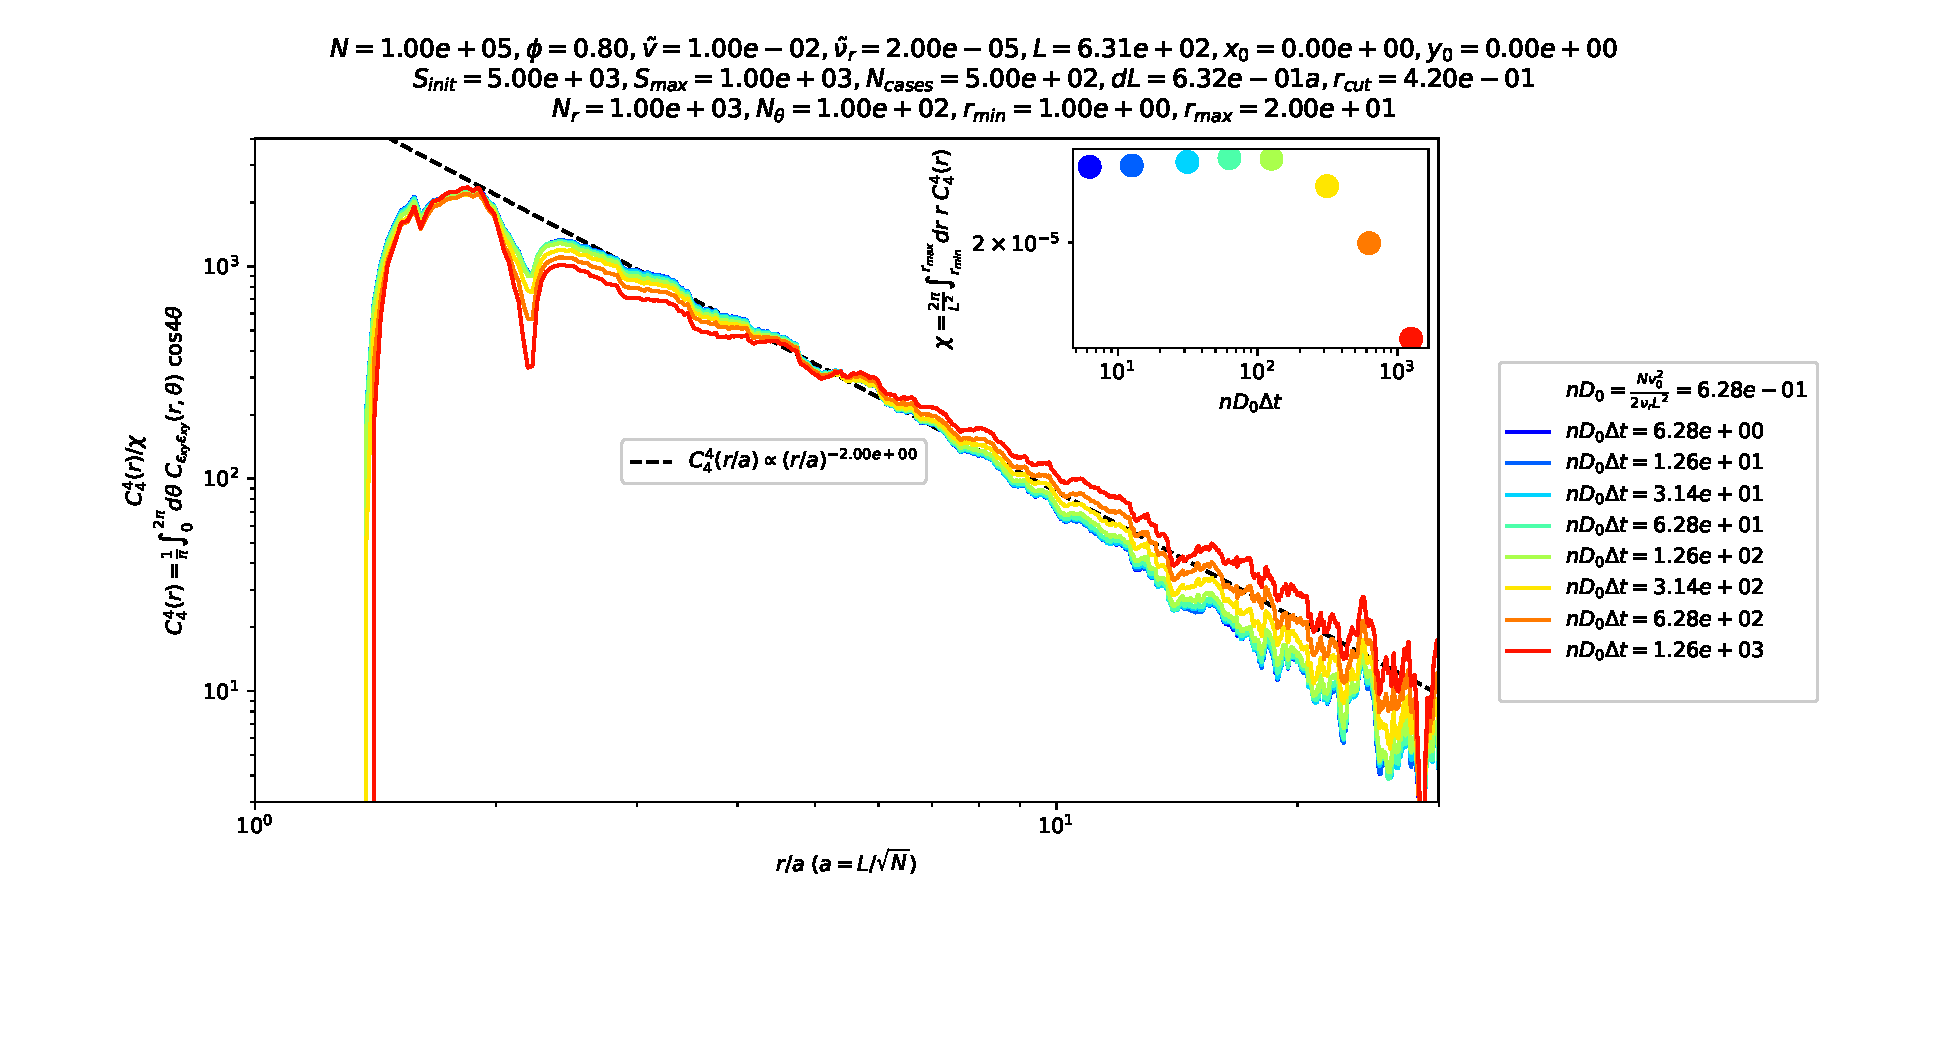
\includegraphics[width=\textwidth]{c44_chi_cmsd_comparison_Dk8000_Vj1000_Rg2000_Nq1000_Ll3000_RCUTk4200_interpolated_loglog.eps}
\caption{Projection of shear strain correlations on $\cos4\theta$, $C_4^4(\Delta r, \Delta t)$ according to equation \ref{c44_definition}, normalised by its susceptibility $\chi = \int dr~ 2 \pi r~ C_4^4(r, \Delta t)$, at packing fraction $\phi = 0.80$, self-propelling velocity $\tilde{v} = 1\cdot10^{-2}$, and rotational diffusion rate $\tilde{\nu}_r = 2\cdot10^{—5}$ (phase separated regime), for different lag times $\Delta t$. A linear interpolation between grid boxes has been performed in the step from the shear strain correlation grid to the $C_4^4(\Delta r, \Delta t)$ function to smooth the curve. We have $n = N/L^2$ the number density of particles and $D_0 = V_0^2/2\nu_r$ the diffusion constant of a single particle, introduced for matter of comparison of lag times between different systems as suggested in \cite{illing2016strain}. The dashed line corresponds to an arbitrary fit to a power law $(r/a)^{—2}$.}
\label{c44_cmsd_high}
\end{figure}

We perform the same calculations for a system of lower activity, in the fluid regime. Our results are presented in figure \ref{c44_cmsd_low}.\\

For this system in fluid state, we recover the results of figure \ref{c44_real_fluid}, \textit{i.e.} we have a peak of $C_4^4(\Delta r, \Delta t)$ close to 2 units of average particle separation and curves collapse. Moreover, we observe an exponential decay of the correlations, with a length scale of a few particles and which is an increasing function of increasing lag time $\Delta t$.

\begin{figure}[H]
\centering
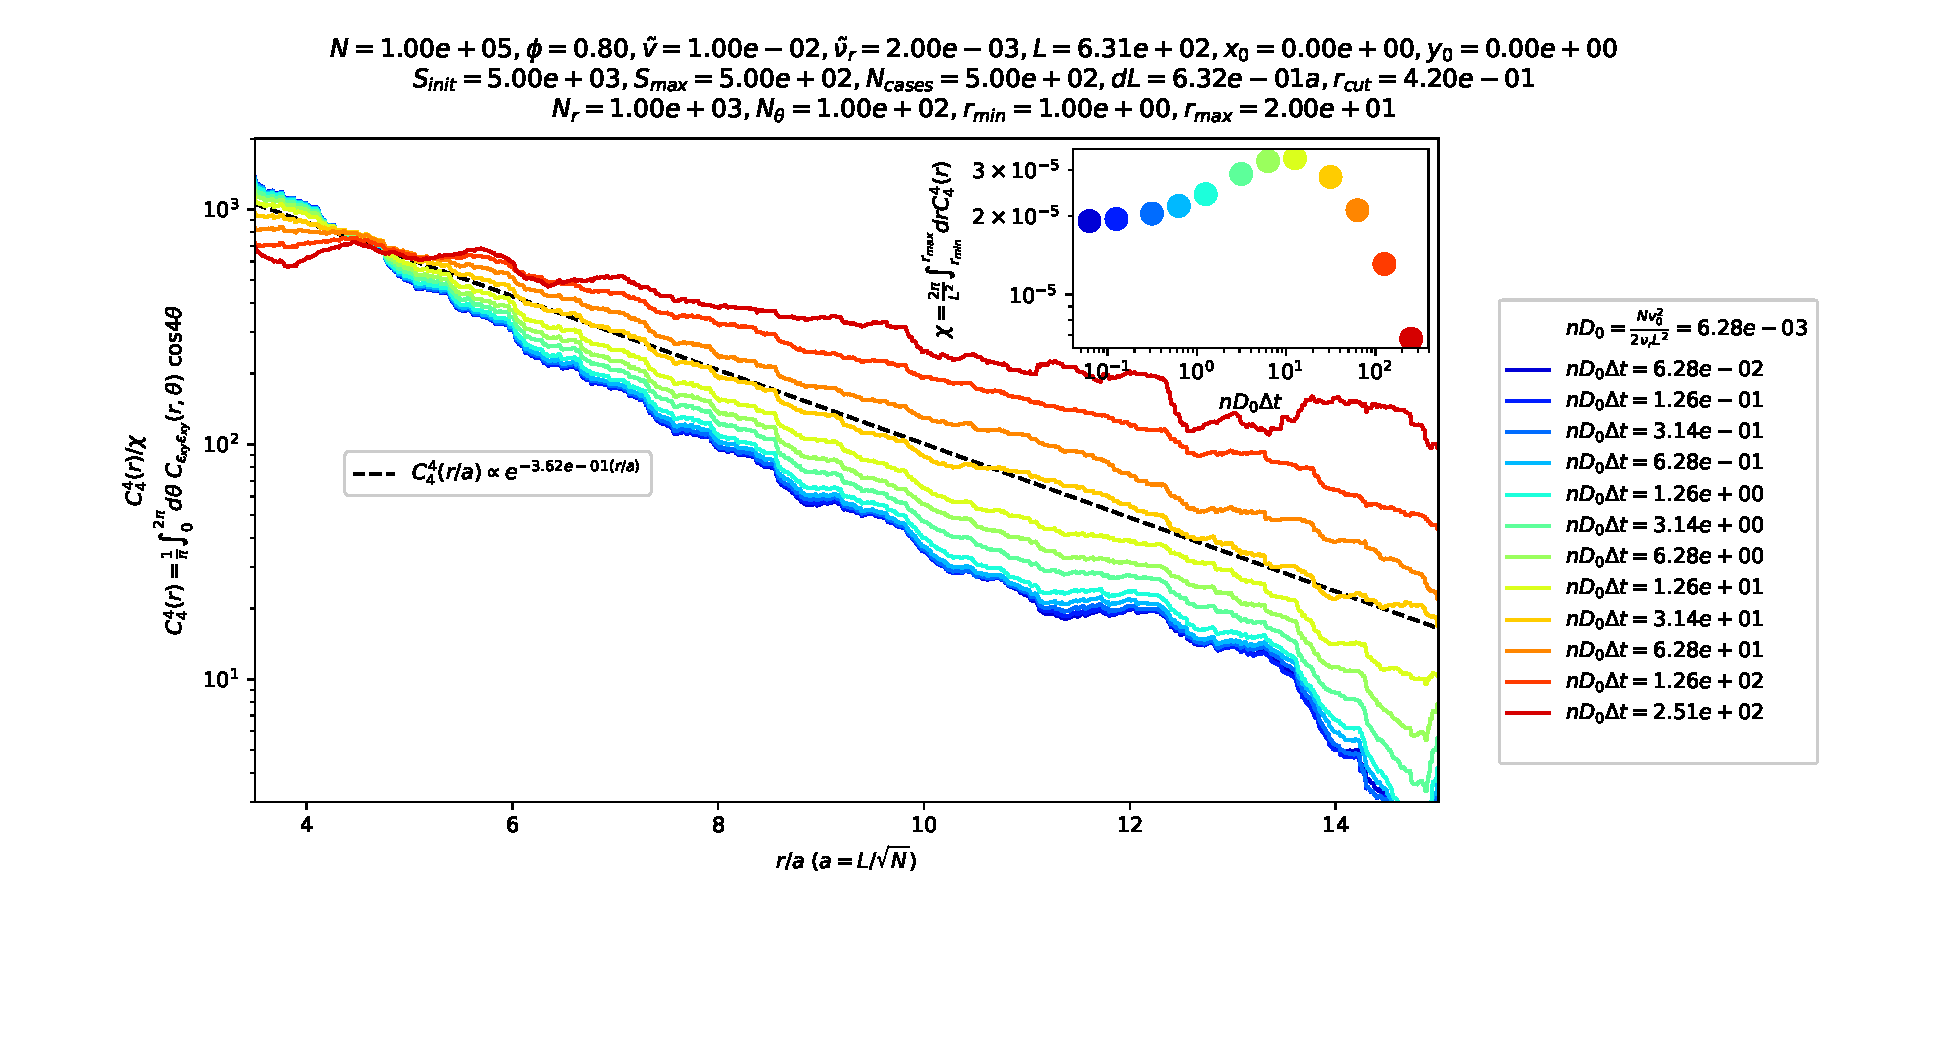
\includegraphics[width=\textwidth]{c44_chi_cmsd_comparison_Dk8000_Vj1000_Ri2000_Nq1000_Ll0000_Mo1000_RCUTk4200_interpolated_linlog.eps}
\caption{Projection of shear strain correlations on $\cos4\theta$, $C_4^4(\Delta r, \Delta t)$ according to equation \ref{c44_definition}, normalised by its susceptibility $\chi = \int dr~ 2 \pi r~ C_4^4(r, \Delta t)$, at packing fraction $\phi = 0.80$, self-propelling velocity $\tilde{v} = 1\cdot10^{-2}$, and rotational diffusion rate $\tilde{\nu}_r = 2\cdot10^{—3}$ (fluid regime), for different lag times $\Delta t$. A linear interpolation between grid boxes has been performed in the step from the shear strain correlation grid to the $C_4^4(\Delta r, \Delta t)$ function to smooth the curve. We have $n = N/L^2$ the number density of particles and $D_0 = V_0^2/2\nu_r$ the diffusion constant of a single particle, introduced for matter of comparison of lag times between different systems as suggested in \cite{illing2016strain}. The dashed line corresponds to an arbitrary fit to an exponential $\exp(-0.362(r/a))$.}
\label{c44_cmsd_low}
\end{figure}

We then conclude here as we have concluded in section \ref{subsection:real_method_results}: more analyses are needed to characterise the transition from exponential to algebraic decay of the shear strain correlations with increasing activity.

\end{document}
